%% This is file `elsarticle-template-1-num.tex',
%%
%% Copyright 2009 Elsevier Ltd
%%
%% This file is part of the 'Elsarticle Bundle'.
%% ---------------------------------------------
%%
%% It may be distributed under the conditions of the LaTeX Project Public
%% License, either version 1.2 of this license or (at your option) any
%% later version.  The latest version of this license is in
%%    http://www.latex-project.org/lppl.txt
%% and version 1.2 or later is part of all distributions of LaTeX
%% version 1999/12/01 or later.
%%
%% The list of all files belonging to the 'Elsarticle Bundle' is
%% given in the file `manifest.txt'.
%%
%% Template article for Elsevier's document class `elsarticle'
%% with numbered style bibliographic references
%%
%% $Id: elsarticle-template-1-num.tex 149 2009-10-08 05:01:15Z rishi $
%% $URL: http://lenova.river-valley.com/svn/elsbst/trunk/elsarticle-template-1-num.tex $
%%
\documentclass[preprint,12pt]{elsarticle}

%% Use the option review to obtain double line spacing
%% \documentclass[preprint,review,12pt]{elsarticle}

%% Use the options 1p,twocolumn; 3p; 3p,twocolumn; 5p; or 5p,twocolumn
%% for a journal layout:
%% \documentclass[final,1p,times]{elsarticle}
%% \documentclass[final,1p,times,twocolumn]{elsarticle}
%% \documentclass[final,3p,times]{elsarticle}
%% \documentclass[final,3p,times,twocolumn]{elsarticle}
%% \documentclass[final,5p,times]{elsarticle}
%% \documentclass[final,5p,times,twocolumn]{elsarticle}

%% if you use PostScript figures in your article
%% use the graphics package for simple commands
%% \usepackage{graphics}
%% or use the graphicx package for more complicated commands
%% \usepackage{graphicx}
%% or use the epsfig package if you prefer to use the old commands
%% \usepackage{epsfig}

%% The amssymb package provides various useful mathematical symbols
\usepackage{amssymb}
%% The amsthm package provides extended theorem environments
%% \usepackage{amsthm}

%% The lineno packages adds line numbers. Start line numbering with
%% \begin{linenumbers}, end it with \end{linenumbers}. Or switch it on
%% for the whole article with \linenumbers after \end{frontmatter}.
\usepackage{lineno}

%% natbib.sty is loaded by default. However, natbib options can be
%% provided with \biboptions{...} command. Following options are
%% valid:

%%   round  -  round parentheses are used (default)
%%   square -  square brackets are used   [option]
%%   curly  -  curly braces are used      {option}
%%   angle  -  angle brackets are used    <option>
%%   semicolon  -  multiple citations separated by semi-colon
%%   colon  - same as semicolon, an earlier confusion
%%   comma  -  separated by comma
%%   numbers-  selects numerical citations
%%   super  -  numerical citations as superscripts
%%   sort   -  sorts multiple citations according to order in ref. list
%%   sort&compress   -  like sort, but also compresses numerical citations
%%   compress - compresses without sorting
%%
%% \biboptions{comma,round}

% \biboptions{}

\pdfinclusioncopyfonts=1 

\journal{Environmental and Ecological Modelling}

\begin{document}


\begin{frontmatter}

%% Title, authors and addresses

%% use the tnoteref command within \title for footnotes;
%% use the tnotetext command for the associated footnote;
%% use the fnref command within \author or \address for footnotes;
%% use the fntext command for the associated footnote;
%% use the corref command within \author for corresponding author footnotes;
%% use the cortext command for the associated footnote;
%% use the ead command for the email address,
%% and the form \ead[url] for the home page:
%%
%% \title{Title\tnoteref{label1}}
%% \tnotetext[label1]{}
%% \author{Name\corref{cor1}\fnref{label2}}
%% \ead{email address}
%% \ead[url]{home page}
%% \fntext[label2]{}
%% \cortext[cor1]{}
%% \address{Address\fnref{label3}}
%% \fntext[label3]{}

\title{Spatial modelling of rice yield losses in Tanzania due to bacterial blight and leaf blast in a changing climate} 

%% use optional labels to link authors explicitly to addresses:
%% \author[label1,label2]{<author name>}
%% \address[label1]{<address>}
%% \address[label2]{<address>}

\author[AfricaRice, WUR]{C. Duku}
\ead{confidence.duku@wur.nl}
\author[IRRI]{A.H. Sparks}
\ead{a.sparks@irri.org}
\author[AfricaRice]{S.J. Zwart\corref{cor1}}
\ead{s.zwart@cgiar.org}
\author[IRRI]{J.K. Aunario}
\ead{j.aunario@irri.org}

\cortext[cor1]{Corresponding author}

\fntext[fn1]{Current address: } 
\address[AfricaRice]{Africa Rice Center (AfricaRice), 01 BP 2031, Cotonou, BENIN}
\address[WUR]{Somewhere in Europe}
\address[IRRI]{International Rice Research Institute (IRRI), DAPO Box 7777, Metro Manila, 1301, PHILIPPINES}

\begin{abstract}

\end{abstract}

\begin{keyword}
bacterial blight \sep leaf blast \sep EPIRICE \sep RICEPEST \sep crop modelling
\end{keyword}

\end{frontmatter}



%%
%% Start line numbering here if you want
%%
\linenumbers

%% main text
\section{Introduction}
Rice is the most rapidly growing staple food in Africa and although rice production is steadily increasing, the consumption is still outpacing the production. For example by 2009 37 per cent of the rice consumed in Africa was imported. To reduce its reliance on imports and dependency on global markets Africas rice production needs to increase further \cite{Seck2013}. Current average yield levels in Africa range from about 1 t ha\textsuperscript{-1} in upland ecologies to 1.5 to 2 t ha\textsuperscript{-1} in rain fed lowland ecologies with the irrigated lowland ecologies having the highest yields of 3.0 to 4.0 t ha\textsuperscript{-1} \cite{Diagne2013}. Rice yields in African farmers fields are low due to a combination of abiotic and biotic stresses that constrain them. Farmers can significantly reduce the yield gaps with improved field, water and crop management, and weed control \cite{Saito2013}.

Apart from weeds, pests and diseases also are major biotic stresses that can cause significant reductions in rice yields. Two important diseases in Sub-Saharan African rice are leaf blast (LB), causal agent \textit{Magnaporthe oryzae}, and bacterial blight (BB) \cite{Verdier2012}, causal agent \textit{Xanthamonas oryzae} pv. \textit{oryzae}. Because infectious plant disease occurs as an interaction of a favorable environment, a susceptible host and a competent pathogen \cite{Madden2007}, weather conditions impact both the occurrence and gravity of plant disease. Climate change is likely to affect plant disease \cite{Anderson2004, Coakley1999, Garrett2006} and several others have expressed interest in changes to plant disease as a result of climate change \cite{Chakraborty2011, Juroszek2011, Luck2011, Pautasso2010, Savary2011, Sutherst2011}. Moreover, intensification of rice production, which was witnessed in Sub-Saharan Africa since the food crisis of 2008 \cite{Saito2013}, may lead to an increased yield loss due to the blast, thus reducing the benefits that were created \cite{Sere2013}. Increases in disease incidence and severity may deter farmers from investing in intensification measures because of risks related to yield losses or even total crop failure. To the authors knowledge, the impact of climate change on leaf blast and bacterial blight diseases of rice in Africa has not yet been investigated.

Efforts to link plant disease models with a geographic information system (GIS) to assess the impact of plant diseases spatially include  \citet{Hijmans2000}, which mapped the global number of pesticide applications necessary to control potato late blight using contemporary weather data. While Sparks et al. (2014) used a meta-model to generate map estimates of changes in global potato late blight due to climate change. \citet{Savary2012} developed a GIS-linked model, EPIRICE, capable of simulating several important diseases of rice, including leaf blast and bacterial blight amongst others.

The objective of the study was to quantify the impact of climate change as forecasted by the Intergovernmental Panel on Climate Change (IPCC) on rice yield loss as result of BB and LB. To carry out this study, we linked two previously unlinked, existing models, EPIRICE and RICEPEST \cite{Willocquet2000, Willocquet2002}, and we applied them using spatially and temporally downscaled climate change data to generate predictions on changes in plant disease impact due to climate change in Tanzania.

Rice accounts for five percent of the total value of agricultural production in Tanzania and is the 7th most important agricultural crop with steadily increasing production over the last decade. However, rice yields in Tanzania remain significantly lower than in neighboring countries \cite{Barreiro-Hurle2012}.

The RICEPEST model has been used to estimate yield losses due to diseases and other pest injuries in rice in varying production situations, but until now these estimates have not been geographically representable. Additionally, the previous use of the RICEPEST model included only weather data that varied. The levels of disease damages were limited to the original levels of disease that corresponded to observations that were taken during model development or chosen by the user. Using EPIRICE output allows us to obtain spatial and temporal estimates of yield losses due to disease as affected by conducive weather.

This paper will continue with a justification for the study area, followed by descriptions of the EPIRICE and RICEPEST models. We will then elaborate the framework for assessing rice yield losses under climate change that links both models. The procedure for generating daily weather inputs from the downscaled climate scenarios is outlined followed by the choice of production situations. Next the results are presented, followed by a discussion and finally conclusions.


\section{Materials and Methods}

%Rice (importance, areas, growing seasons)
%Current climate 
%Climate change impact (growing seasons?)

\subsection{The study region}
Tanzania was chosen as the study region because of its location in sub-Saharan Africa, the probabal effects of climate change in the region and rice is planted widely across the country \cite{Rowhani2011} (Table 1). The bulk of the rice crop is grown from December until June of the following year during the rainy season. According to the International Panel on Climate Change (IPCC), East Africa and especially the Great Lakes Region are among the more vulnerable regions in Africa to climate change, where the trend is towards increasing temperatures and declining rainfall according to General Circulation Model outputs \cite{Boko2007}.

\subsection{Model descriptions}
\subsubsection{The EPIRICE model}
EPIRICE \cite{Savary2012} is a SEIR (susceptible-exposed-infectious-removed) model implemented in R  \cite{R2014} that simulates potential spatial epidemics of rice diseases including BB and LB. Model inputs are date of crop establishment and daily time-step climate data, precipitation, maximum and minimum temperature, and relative humidity. The model as originally implemented produces a single aggregated output, a map, at the end of a growing season of a measure called Area Under Disease Progress Curve (AUDPC) \cite{Shaner1977}. However, for this study, daily disease severity expressed as a percentage was generated for use in the RICEPEST model, which we discuss further in a later portion of this paper.

\subsubsection{The RICEPEST model}
The RICEPEST model \cite{Willocquet2000, Willocquet2002} simulates rice yield losses due to several yield-reducing factors under a range of specific production situations with simulated diseases including BB and LB. The model runs on a daily time-step with simulation starting 14 days after crop establishment for both transplanted and direct seeded rice. The model incorporates two sub-models, the first sub-model simulates the dynamics of the rice crop biomass and the second sub-model simulates the dynamics of the tiller population. The biomass sub-model accounts for the daily accumulation and partitioning of assimilates towards roots, leaves, stems, and panicles. For this study, because the damage mechanisms of the diseases of interest (BB and LB) are simulated only in the biomass sub-model, the tiller sub-model was not considered.

Bacterial blight and LB cause lesions on the leaf blades. These lesions decrease the green leaf area index (LAI), reducing the photosynthetic capacity of the plant. To account for this, the RICEPEST model uses a reduction factor to reduce the value of LAI and subsequently the overall rate of growth (RG) \cite{Willocquet2002}. 
\begin{equation}
(1  (BBDM_t / 100)
\end{equation}

\begin{equation}
(1  (LBDM_t / 100))
\end{equation}

\begin{equation}
LAI_t = SLA_t  LEAFWt  (1  (BBDM_t / 100)) 
\end{equation}
 
\begin{equation}
RG_t = RUE_t  RAD_t  (1- exp(- k  LAI_t))
\end{equation}

BBDM and LBDM are the percent of leaf area covered by BB and LB respectively \cite{Willocquet2002}. SLA is the specific leaf area; LEAFW is the leaf dry weight; RUE is radiation use efficiency; RAD is daily solar radiation; k is coefficient of light extinction 
\begin{equation}
(1- exp( - k  LAI_t)
\end{equation}
and is the proportion of light intercepted by the crop, set to 0.6 \cite{Willocquet2000}.

Three different injury profiles as listed in Table 2 were defined for this study. The defined production situation was then treated with these injury profiles to obtain the actual yield for each treatment combination.

\subsubsection{Model coupling}
To facilitate coupling of EPIRICE to RICEPEST, a temporal disaggregation function was incorporated into the EPIRICE model. With this function, the modified EPIRICE model produced daily, spatially representative and non-cumulative percentage disease severity data as outputs instead of the single cumulated output, AUDPC. The time-series of daily percentage disease severity data for BB and LB produced by the modified EPIRICE model were then used as inputs for RICEPEST. Both models were linked to a geographic information system (GIS). EPIRICE is implemented in the R language using the following packages: cropsim \cite{Hijmans2009}, oldweather \cite{Hijmans2009}, raster \cite{Hijmans2014}, rgdal \cite{Bivand2014}, and RODBC \cite{Ripley2013}, while this version of RICEPEST is implemented in Python language, using the ArcPy package, as a script in the ArcGIS platform \cite{ESRI2011}. Due to the different implementation environments, a loose coupling approach was therefore adopted. A loose coupling approach provided flexibility in data handling and data interoperability. 

\subsection{Growing seasons and areas}
A planting window of late November to early December, the major growing season for most rain-fed ecologies in Tanzania according to the FAO cropping calendar (citation), was selected and ArcGIS was used to create a spatial dataset of areas with this planting window. Annual harvested rain-fed rice growing areas for Tanzania with values representing the proportion of harvested areas (in hectares) within each pixel (10,000ha) was also obtained from MIRCA2000 \cite{Portmann2010}. To select the major rice growing areas in Tanzania during this planting window, a simple raster overlay analysis was performed in ArcGIS.

\subsection{Weather Data Generation}
For this study, the General Circulation Model (GCM), Commonwealth Scientific and Industrial Research Organization Mark 3 (CSIRO-MK3) was selected. Downscaled outputs from this GCM based on three future climate scenarios A1B, A2 and B1 as reported in the Special Report on Emission Scenarios (SRES) of the IPCC Fourth Assessment Report, for two time slices 2030s (2021-2040) and 2050s (2041-2060) were obtained. A2 is a high greenhouse gas emission scenario; A1B, a medium-emission scenario; and B1, a low-emissions scenario. The selection of the GCM and the emission scenarios were based on the availability of complete downscaled climate data to run both models. Monthly projected precipitation, minimum and maximum temperature, solar radiation and wet day frequency outputs of this GCM, spatially downscaled to approximately 10km grid resolution using a pattern scaling approach were obtained from CIAT CCAFS Geoportal (http://www.ccafs-climate.org) \cite{Jones2009}. Relative humidity outputs of this GCM were however obtained directly from the CMIP3 dataset and spatially downscaled to 10km using statistical downscaling delta technique. Observed climate data for the period 2000s (1991-2010) was obtained from the same source and used as the baseline for this study. A parametric stochastic weather generator, MODAWEC \cite{Liu2009}, which requires only monthly data (as outlined in \citet{Geng1986} and MODAWEC) was used to generate daily precipitation, maximum and minimum temperature datasets corresponding to future scenarios. This was essential in producing daily minimum and maximum temperature data that correlate with precipitation. A linear interpolation technique was, however, used in generating daily relative humidity and solar radiation from monthly data. The daily weather data generated were used as inputs in both EPIRICE and RICEPEST models.

\subsection{Production situations}
Production situations directly affect the intensity of rice yield reduction for a given injury profile \cite{Savary2000}. For this study, production situation is defined as the combination of socioeconomic, environmental and biophysical factors excluding pests that define the attainab1e yield. Temperature and solar radiation were excluded from this definition because they remain unchanged across all the possible production situations in the study area. Due to lack of reliable information about the spatial arrangement of production situations in the study area, the production situation was assumed to be homogenous based on the most common production situation, lowland rainfed rice \cite{Diagne2013} (Table 1). The production situation was characterized using the following parameters: a rice cultivar of 90 days to flowering and 120 days to maturity, crop establishment type was direct seeded, fertilizer input or nitrogen management was 180kg/ha and the water management was a rainfed system with fairly good water management. Using data from farmer surveys, literature review and expert opinion, a number of production situations were defined for rice growing ecologies. However, lowland rainfed, direct seeded rice was the most common production situation, so it  was selected for this study and production situation was considered to be homogenous within the entire study area. 

Comparing this with previous work by \citet{Willocquet2002}, the selected production situation was translated into quantitative estimates of leaf (LEAFW), stem (STEMW) and root (ROOTW) dry weights after 14 DACE. Panicle dry weight (PANW) after 14 DACE was however set to zero. These values were then used to initialize the model for simulations. 

\subsection{Spatial modelling of yield loss}
Simulation runs EPIRICE and RICEPEST were made separately at a spatial resolution of 10km\textsuperscript{2} for the growing season December to March. Outputs of daily non-cumulative percentage disease intensity in GeoTIFF format were then produced for each climate scenario in the 2030 and 2050 time slices. Simulation runs were also made for current climate conditions.

To map and quantify the spatial distribution of rice yield loss as a result of the two diseases under current and future climate conditions, the RICEPEST model was linked to weather data (temperature and solar radiation) and disease severity outputs from the EPIRICE model within the ArcGIS environment using the aforementioned Python tool. Simulation runs were first made without the injury profiles to obtain the attainable yield. Maintaining the same weather data and production situation parameter values, simulation runs were then made with the treatment of injury profiles to obtain the actual yield in the presence of the two diseases, separately. Yield loss was then modelled as the difference between attainable yield and actual yield for both BB and LB.

\section{Results and discussion}

\subsection{Potential epidemics (EPIRICE output)}
Bacterial blight epidemics in all time slices and scenarios started rapidly increasing around day 50 and increases up until day 100, when it begins decreasing 

\subsection{Yield losses (RICEPEST output)}

\section{Conclusions}

\section{Acknowledgements}
MICCORDEA project financed by GIZ, CCAFS and GRiSP consortium research programs


%% The Appendices part is started with the command \appendix;
%% appendix sections are then done as normal section
\appendix

\section{Figures}
\label{Figures}
\begin{figure}[htb]
  \caption{Bacterial leaf blight disease severity curves.}
  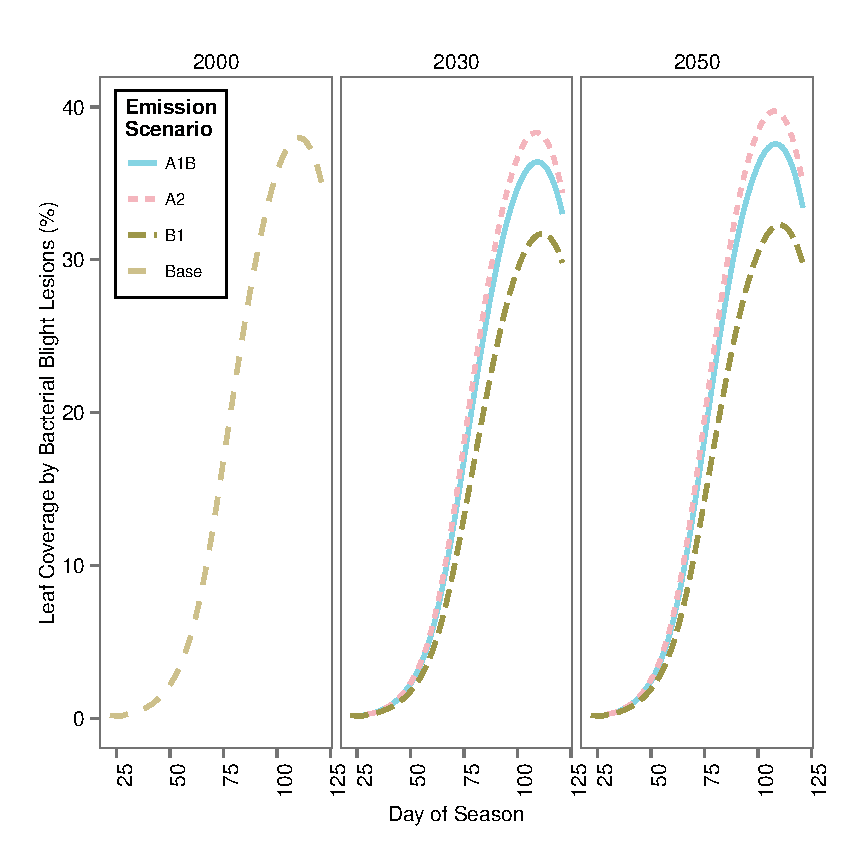
\includegraphics[width = 1\textwidth]{figures/BB}
\end{figure}


%% References
%%
%% Following citation commands can be used in the body text:
%% Usage of \cite is as follows:
%%   \cite{key}          ==>>  [#]
%%   \cite[chap. 2]{key} ==>>  [#, chap. 2]
%%   \citet{key}         ==>>  Author [#]

%% References with bibTeX database:

\bibliographystyle{elsarticle-num-names}
\bibliography{MICORDEA_References}

%% Authors are advised to submit their bibtex database files. They are
%% requested to list a bibtex style file in the manuscript if they do
%% not want to use model1-num-names.bst.

%% References without bibTeX database:

% \begin{thebibliography}{00}

%% \bibitem must have the following form:
%%   \bibitem{key}...
%%

% \bibitem{}

% \end{thebibliography}


\end{document}

%%
%% End of file `Duku et al.tex'.
